\documentclass[]{book}

%These tell TeX which packages to use.
\usepackage{array,epsfig}
\usepackage{amsmath}
\usepackage{amsfonts}
\usepackage{amssymb}
\usepackage{amsxtra}
\usepackage{amsthm}
\usepackage{mathrsfs}
\usepackage{color}
\usepackage{graphicx}
\usepackage{float}

%Algorithm packages
\usepackage{algorithm}  
\usepackage{algpseudocode}  
\usepackage{amsmath}  
\renewcommand{\algorithmicrequire}{\textbf{Input:}}  % Use Input in the format of Algorithm  
\renewcommand{\algorithmicensure}{\textbf{Output:}} % Use Output in the format of Algorithm  
%Here I define some theorem styles and shortcut commands for symbols I use often
\theoremstyle{definition}
\newtheorem{defn}{Definition}
\newtheorem{thm}{Theorem}
\newtheorem{cor}{Corollary}
\newtheorem*{rmk}{Remark}
\newtheorem{lem}{Lemma}
\newtheorem*{joke}{Joke}
\newtheorem{ex}{Example}
\newtheorem*{soln}{Solution}
\newtheorem{prop}{Proposition}

\newcommand{\lra}{\longrightarrow}
\newcommand{\ra}{\rightarrow}
\newcommand{\surj}{\twoheadrightarrow}
\newcommand{\graph}{\mathrm{graph}}
\newcommand{\bb}[1]{\mathbb{#1}}
\newcommand{\Z}{\bb{Z}}
\newcommand{\Q}{\bb{Q}}
\newcommand{\R}{\bb{R}}
\newcommand{\C}{\bb{C}}
\newcommand{\N}{\bb{N}}
\newcommand{\M}{\mathbf{M}}
\newcommand{\m}{\mathbf{m}}
\newcommand{\MM}{\mathscr{M}}
\newcommand{\HH}{\mathscr{H}}
\newcommand{\Om}{\Omega}
\newcommand{\Ho}{\in\HH(\Om)}
\newcommand{\bd}{\partial}
\newcommand{\del}{\partial}
\newcommand{\bardel}{\overline\partial}
\newcommand{\textdf}[1]{\textbf{\textsf{#1}}\index{#1}}
\newcommand{\img}{\mathrm{img}}
\newcommand{\ip}[2]{\left\langle{#1},{#2}\right\rangle}
\newcommand{\inter}[1]{\mathrm{int}{#1}}
\newcommand{\exter}[1]{\mathrm{ext}{#1}}
\newcommand{\cl}[1]{\mathrm{cl}{#1}}
\newcommand{\ds}{\displaystyle}
\newcommand{\vol}{\mathrm{vol}}
\newcommand{\cnt}{\mathrm{ct}}
\newcommand{\osc}{\mathrm{osc}}
\newcommand{\LL}{\mathbf{L}}
\newcommand{\UU}{\mathbf{U}}
\newcommand{\support}{\mathrm{support}}
\newcommand{\AND}{\;\wedge\;}
\newcommand{\OR}{\;\vee\;}
\newcommand{\Oset}{\varnothing}
\newcommand{\st}{\ni}
\newcommand{\wh}{\widehat}

%Pagination stuff.
\setlength{\topmargin}{-.3 in}
\setlength{\oddsidemargin}{0in}
\setlength{\evensidemargin}{0in}
\setlength{\textheight}{9.in}
\setlength{\textwidth}{6.5in}
\pagestyle{empty}



\begin{document}


\begin{center}
{\Large COMP 540 \hspace{0.5cm} HW 5}\\
\textbf{Peiguang Wang, Xinran Zhou}\\ %You should put your name here
Due: 3/5/2018 %You should write the date here.
\end{center}

\vspace{0.2 cm}


\subsection*{1: Deep neural networks }
\begin{enumerate}
	\item Why do deep neural networks typically outperform shallow networks?
	\begin{soln}
		By using deep neural network and adding more layers, we can approximate function using less parameters.
		The deep network encodes a set of prior beliefs about the structure of the function we want to learn. Thus, the deep nerual networks reduce the amount of data we should use to get a satisfying result.
	\end{soln}
	\item What is leaky RELU activation and why is it used?
	\begin{soln}
		Leaky relu is basically based on relu activation function and tries to fix the 'dying' problem of relu. When $x<0$, the leaky relu has a small slope instead of being zero.\\
		The reason why we use leaky relu is that it can give a small constant gradient when the input falls in the region $x<0$. So it can fix the problem of "dead relu". 
	\end{soln}
	\item In one or more sentences, and using sketches as appropriate, contrast: AlexNet, VGGNet, GoogleNet and ResNet. What is the one defining characteristic of each network?
	\begin{soln}
		AlexNet: AlexNet uses RELU activate function instead of sigmoid function for the first time. And it also introduce a new dropout layer in the network.
		
		VGGNet: VGGNet consists of either 16 or 19 convolutional layers and has very uniform architecture.
		
		GoogleNet: This module is based on several very small convolutions in order to drastically reduce the number of parameters. 
		
		ResNet: ResNet introduces a so called "shortcut connection" that skips one or more layers, which allow the gradients can be backprop to the first layers. This allows us to train a much deeper network up to 152 layers.
	\end{soln}
	
\end{enumerate}
\subsection*{2: Decision trees, entropy and information gain }
	\begin{enumerate}
		\item  Show that $H(S) ≤ 1$ and that $H(S) = 1$ when $p = n$.
		\begin{soln}
			Since
			$$H(q) = - q log(q)- (1-q)log(1-q)$$
			the second derivative of the $-H(q)$ is non-negative, so the negative entropy is convex. The $H(q)$ is concave. The maximum can be obtained at $\frac{\partial H }{\partial q } = 0$
			$$\frac{\partial H }{\partial q } = -log(q) +log(1-q)$$
			thus we got $q = 0.5$, which means that $p = n$ and $H(S) = 1$.
			
			Therefore, $H(S) ≤ 1$ and that $H(S) = 1$ when $p = n$.
			
		\end{soln}
		\item Calculate the reduction in cost using misclassification rate, entropy, and Gini index for models A and B. Which is the preferred split (model A or model B) according to these cost calculations?
		\begin{soln}
			\textbf{Misclassification rate:}
			$$error_A = \frac{100 + 100 }{400+400} = 0.25$$
			$$error_B = \frac{200}{400+400} = 0.25$$ 
			
			\textbf{Entropy:} 
			For both A and B:
			$$H(D) = 1$$
			For A:
			$$H(D_1) =H(D_2) =  - 0.75 log(0.75) - 0.25log(0.25) = 0.811$$
			$$g(D,A) = H(D) -0.5H(D_1) - 0.5H(D_2) = 0.189$$
			For B:
			$$H(D_1) = - \frac{1}{3}log(\frac{1}{3}) - \frac{2}{3}log(\frac{2}{3}) = 0.913$$
			$$H(D_2)= 0$$
			$$g(D,B) = H(D)-0.75H(D_1)-0.25H(D_2) = 0.312$$
			
			\textbf{Gini Index:}
			$$Gini(A) = 0.5(1-0.75^2 - 0.25^2) + 0.25(1-0.25^2 - 0.75^2) = 0.375$$
			$$Gini(B) = 0.75(1-\frac{2}{3}^2 - \frac{1}{3}^2)+0.25(1-1-0)=\frac{1}{3}$$
			Among these three cost calculations, the entropy is the preferred split since the difference between A and B in this cost calculation is the biggest.
		\end{soln}
		\item Can the misclassification rate ever increase when splitting on a feature? If so, give an example. If not, give a proof.
		\begin{soln}
			No, the misclassification rate will not increase when splitting on a feature. 
		\end{soln}
	\end{enumerate}
\subsection*{3: Bagging }
	\begin{enumerate}
		\item Assuming that the individual errors $\epsilon_l$(x) have zero mean and are uncorrelated, that is $E_x[\epsilon_l (x)] = 0$ and $E_x[\epsilon_m (x)\epsilon_l (x)] = 0$ for $m \neq l $, show that
		$$ E_{bag} = \frac{1}{L} E_{av}$$
		\begin{soln}
			Since 
			$$\epsilon_{bag} = \frac{1}{L}\sum_{l=1}^{L}(f(x)+\epsilon_l(x)) - f(x)$$
			where $\epsilon_l ~ N(\mu,\sigma_l ^2)$, and they are uncorrelated 
			If we calculate the $ E_{bag}$, then
			$$E_{bag} = E[\epsilon_{bag}(x)^2] = var(\epsilon_{bag}(x))$$
			the result is $\frac{1}{L^2}\sum_{l=1}^{L} \sigma_L ^2$
			And we have
			$$E_{av} = \frac{1}{L}\sum_{l=1}^{L}E_x[\epsilon_l(x)^2]$$
			Therefore $E_{bag} = \frac{1}{L}E_{av}$
		\end{soln}
	\item  Show that the average expected squared-error $E_{av}$ of the individual functions and the expected error of bagging $E_{bag}$ satisfy $E_{bag} \leq E_{av}$
	\begin{soln}
		Using Jensens inequality for the special case of convex function $f(x) = x^2$, and we suppose $\lambda_l = \frac{1}{L}$
		$$\sum_{l =1}^{L}\lambda_l f(\epsilon_l) = \frac{1}{L}\sum_{l = 1}^{L}\epsilon_l^2$$
		and according to Jensen's inequality,
		$$\sum_{l =1}^{L}\lambda_l f(\epsilon_l) \geq f(\sum_{l =1}^{L}\lambda_l \epsilon_l) = (\frac{1}{L}\sum_{l = 1}^{L}\epsilon_l^2)^2$$
		so
		$$\frac{1}{L}\sum_{l = 1}^{L}\epsilon_l^2 \geq \epsilon_{bag}^2$$
		therefore
		$$E[\frac{1}{L}\sum_{l = 1}^{L}\epsilon_l^2] \geq E[\epsilon_{bag}^2]$$
		take the expectation on both sides $E_av \geq E_bag $
	\end{soln}
	\end{enumerate}

\subsection*{4: Fully connected neural networks and convolutional neural networks  }
\begin{enumerate}
	\item \textbf{Problem 4.1.7: Multilayer network} \\
	Do the initial losses seem reasonable? 
	\begin{soln}
	The initial loss computed by program is: 
	
	\textit{Running check with reg =  0 \\Initial loss:  2.30808329607 \\Running check with reg =  3.14 \\Initial loss:  6.8866804054 	}
	
	It is reasonable. When reg = 0, Initial loss = $ln(num of classes) = ln(10) = 2.3$. This result corresponds with the computed value. And when reg = 3.4, loss with become larger than loss without regularization.
	
	\end{soln}
	\item \textbf{Problem 4.1.7: Multilayer network} \\
	Did you notice anything	about the comparative difficulty of training the three-layer net vs training the five layer net? 
	\begin{soln}
        The 5-layer network is deeper than a 3-layer network, so the backward spread of the gradient will be more difficult(since the gradient will become smaller in deeper layers). So training five-layer net need bigger weight scale in initialization stage. And the learning rate should be higher.
	\end{soln}

	\item \textbf{Problem 4.2.4: Experimenting with fully connected nets with dropout} \\
	Comment on the shape of the training and validation	accuracy plots for networks trained with and without dropout.
	
	Learning history is shown in Figure. \ref{fig:dropout}. We can see from the figure  that using dropout can prevent overfitting and can make the model better when predicting unseen data. When using dropout, training accuracy is lower however validation accuracy is higher. 
	\begin{figure}[H]
		\centering
		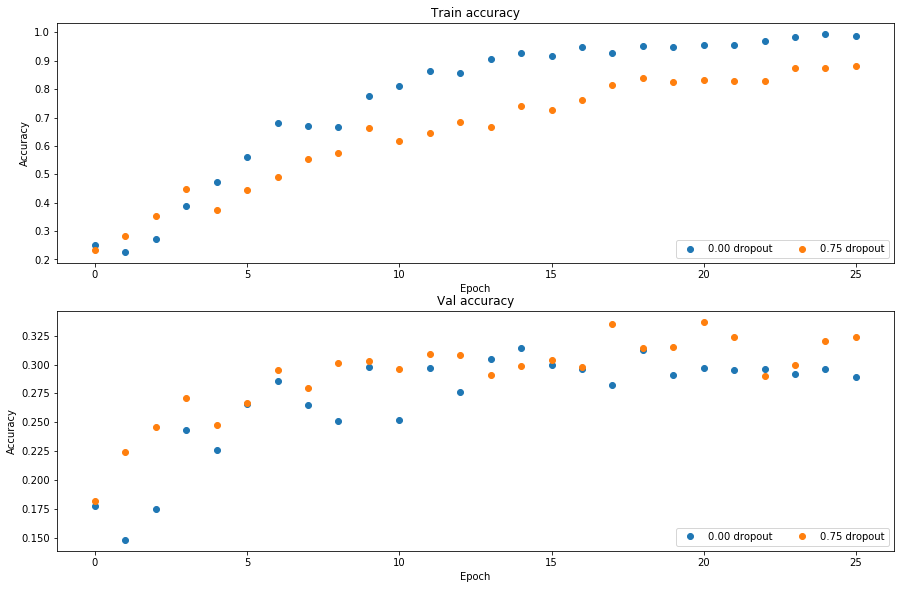
\includegraphics[width=8cm]{dropoutVSnondropout.png}
		\caption{learning history with/without dropout}
		\label{fig:dropout}
	\end{figure}
\end{enumerate}

\end{document}


